\documentclass[journal]{IEEEtran}

\renewcommand{\baselinestretch}{1.0} % Change to 1.65 for double spacing
 
\usepackage{amsmath,amsfonts,amssymb}
\usepackage{graphicx}
\usepackage[colorlinks=true, allcolors=blue]{hyperref}


\usepackage{color}
\usepackage[latin9]{inputenc}
\usepackage{mathrsfs,amsmath}
\usepackage{graphicx}%
\usepackage{float}
\usepackage{amsfonts}%
\usepackage{amssymb}
\usepackage{braket}
\usepackage{bm}
%necessary for outline section of the article 
\usepackage{outline}

\newcommand{\mb}[1]{\bm{#1}}
\usepackage[T1]{fontenc}

\def\Nabla{\bm{\nabla}}
\def\bm{\mathbf}
\def\curl{\Nabla\times}
\def\div{\Nabla\cdot}
\def\lap{\Delta}
\def\vlap{\Delta}
\def\x{\hat{e}_{x}}
\def\y{\hat{e}_{y}}
\def\z{\hat{e}_{z}}
\def\p{\partial}
\def\h{\hat}
\def\tw{\tilde{\omega}}
\def\gm{\gamma}
\def\om{\omega}
\def\OM{\Omega}
\def\GM{\Gamma}
\def\dw{\delta\omega}
\def\dth{\Delta\theta}
\def\dk{\delta k}
\def\Hdth{\frac{\dth}{2}} %half Delta Theta

\DeclareMathOperator{\Tr}{Tr}


\title{Temporal Hole Burning in QCLs with Strong Injector Anticrossing}
\author{\IEEEauthorblockN{Petar Tzenov\IEEEauthorrefmark{1},
		David Burghoff\IEEEauthorrefmark{2},
		Qing Hu\IEEEauthorrefmark{2}, 
		Christian Jirauschek\IEEEauthorrefmark{1}}
	
	\IEEEauthorblockA{\IEEEauthorrefmark{1}Institute for Nanoelectronics, Technical University of Munich, D-80333 Munich, Germany}
	
	\IEEEauthorblockA{\IEEEauthorrefmark{2}Department of Electrical Engineering and Computer Science, Research Laboratory of Electronics, Massachusetts Institute of Technology, Cambridge, Massachusetts 02139, USA}
	\thanks{Corresponding author: P. Tzenov (email: petar.tzenov@tum.de ).}}



\IEEEtitleabstractindextext
 
\begin{document} 
\maketitle

	

\begin{abstract}
The abstract is the last section of your article to be written
because it is a condensed version of the entire article. It
includes the key points of the introduction, methods and
results, and conclusions. An abstract is generally 100?250
words long. It is written in the past tense. An abstract should
not include references; use the background and conclusions
to help frame the context of your work [9].
Readers will use the abstract to decide if your article is relevant
to them. Use keywords and index terms in your abstract to
capture reader interest and improve the likelihood of your article
appearing in relevant searches [3]. Readers who find your article
through an abstracting service may never see the rest of your
article. Be sure the abstract conveys why your research problem
is important and how your work moves the field forward.
Reviewers also look at the abstract first. Strive to make a good
impression with your abstract to engage their attention.
\end{abstract}

\begin{outline}
\item {Introduction}
\begin{outline}
	\item {Short introduction to spatial and spectral hole burning. Sell this as the last out of a group of effects} 
	\item {Short description of the problem formulation -> where was it first reported and what are the specific characteristics of THB} 
	\item {Previous research and literature overview}
\end{outline}
\item{ Experimental Evidence} 
\begin{outline}
	\item {Cite David's original papers}
	\item {Give details about the nature of the experimental measurements and data post-processing involved}
	\item {Show experimental data -> time domain and spectra}  
\end{outline}	
\item{Model Description and Results}
\begin{outline}
	\item { Outline the theoretical model -> comparison between dressed state and TB states picture}
	\item { THB ansatz and system of equations }
	\item { Further insights and parallel with SHB -> travelling wave inversion grating}
	\item { Simulation results -> THz-TDs simulations and long time simulation results for fixed parameters but varying bias} 	
\end{outline}
\item{Conclusion}	
\end{outline}
% Include a list of keywords after the abstract 

\section{Introduction}
	\begin{itemize}
		\item {Short introduction to spatial and spectral hole burning. Sell this as the last out of a group of effects} 
		\item {Short description of the problem formulation -> where was it first reported and what are the specific characteristics of THB} 
	\end{itemize}
The Introduction serves to help the reader understand our
three key questions: Why is this a new and important problem?
What has been done before? How does your research bring
significant new understanding to the field? The reader should
find enough information to understand why your research was
necessary, without having to refer to other source material or
published works [7]. The introduction should be concise, no
more than one or two pages. It is written in the present tense.
Your introductory paragraph should start with what is generally
known about your subject. Then move step by step through
more detailed information, ending with a description of the
specific problem or hypothesis your article will discuss. Try to
use an attention-grabbing statement to hook the reader [10]
while being careful not to sensationalize your results.
In the next few paragraphs, refer to the published research to
show what is already known about your subject and why your
work is needed. Do not try to include everything from your
literature review. Your goal is to orient the reader to the most
relevant studies. Explain how each earlier study relates to your
own approach to the problem. Does it have limitations? Does it
make different assumptions [11]? Show your readers how your
study builds upon or is different from this existing work. If you
have published an earlier version of your work, for example as a
conference or journal article, you must explain how the current
study builds upon your own prior work [3].
After you have explained the historical context of your work,
introduce your hypothesis and provide a general description of
the results you have obtained. You will flesh these out more
fully later in the article, but providing an overview here motivates
your audience to read on. At the end of your introduction, tell
the reader how the article is organized. This will allow readers to
move to sections of particular interest, if they wish.
\section{Experimental evidence}

In addition to emitting a stable frequency comb, consisting of more than 70 equidistantly-spaced longitudinal modes, the device in \cite{burghoff2014terahertz} also exhibited other very intriguing properties which deserve a more detailed study. For example, a hole was observed in the signal's spectrum, which separated the lasing frequencies into components distributed around 3.4 THz and 3.8 THz, to which we will refer  as the low and high frequency lobes, respectively. Such a spectral hole burning was attributed and later theoretically confirmed by simulation [cite our optics paper] to be due to the strong tunneling coupling between injector and upper laser level of the active region. Furthermore, a subsequent detailed experimental analysis \cite{burghoff2015evaluating} showed that the prevalent frequency lobe strongly depends on the applied injection current, with the low and high frequency transitions dominating respectively at low and high current densities \cite{burghoff2015evaluating}. Additionally, a Monte-Carlo based algorithm in combination with a novel comb coherence detection technique, the so called shifted wave interference Fourier transform spectroscopy or SWIFTS \cite{burghoff2014broadband}, was used in order to reconstruct the instantaneous intensity and frequency of the signal \cite{burghoff2015evaluating}. The results displayed an intriguing pulse switching behaviour, which was termed "temporal hole burning" (THB) by the authors, and is at the main focus of this article. 
The observed THB effect can be characterized by a transient switching between signals corresponding to the high and low lobes in a manner as to maintain an almost constant total intensity. This process is illustrated in Fig. \ref{fig:img01}b which displays experimental data of the averaged out instantaneous intensity of the low and high frequency lobes of the power spectrum in Fig. \ref{fig:img01}a. For this measurement the laser was supplied with 0.9 A current and was shown to operate in a stable comb regime. From the plots in Fig. \ref{fig:img01}, we immediately see that whereas both signals' intensities are comparable in strength, the high frequency lobe has significantly longer time duration and hence carries more power. In agreement with Parseval's theorem, this is also confirmed by the optical power spectrum in Fig. \ref{fig:img01}a, where we see that significantly more energy is stored in the modes distributed around 3.8 THz as compared to those at 3.4 THz. 
\begin{figure}[h!]
	\begin{center}
		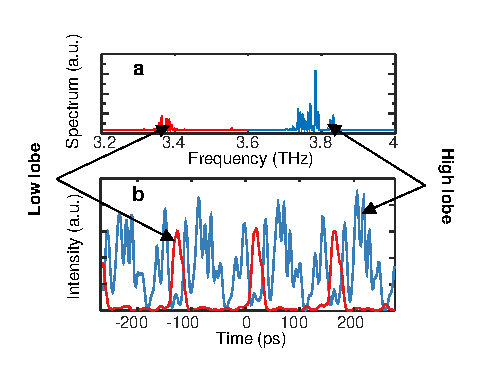
\includegraphics[scale=1.0]{IMGS/THB_experiment.eps}
		\caption{ Insert Caption HERE} \label{fig:img01}
	\end{center}	
\end{figure}
XXX - XXX 

\section{Model description and simulation results}
Consider a prototypical THz QCL design, employing resonant tunneling for efficient current injection, schematically illustrated in Fig.\ref{fig:img02}a. In this configuration, the injector state is denoted as $\ket{c}$, the upper laser level as $\ket{b}$ and the lower laser level as $\ket{a}$. Let us denote the tunneling coupling energy, as $\hslash\Omega_{cb}$, the $b\leftrightarrow c$ detuning energy as $\hslash\epsilon$ and finally the energy of the optical, i.e. $a\leftrightarrow b$, transition as $\hbar \omega_0$. The tunneling coupling between injector and upper laser level leads to a level splitting, i.e. the so called level anticrossing, of the states $\ket{b}$ and $\ket{c}$ into a doublet of dressed states $\ket{+}$ and $\ket{-}$, which span the intramodule barrier, Fig. \ref{fig:img02}b, and are separated by the detuning energy $2\delta\omega = \hslash\sqrt{\epsilon^2 + 4\Omega_{cb}^2}$.  

\begin{figure}[h!]
	\begin{center}
		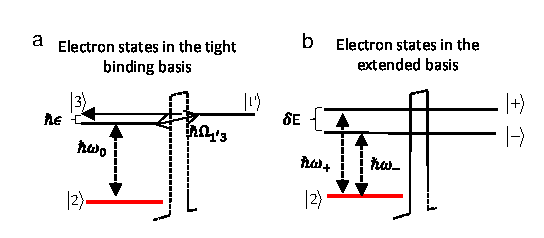
\includegraphics[scale=1.0]{IMGS/basis_compare.eps}
		\caption{ Insert Caption HERE} \label{fig:img02}
	\end{center}	
\end{figure}

The dipole coupling between the states $\ket{b}$ and $\ket{a}$ in the tight binding basis is transferred to a dipole interaction between both dressed states and $\ket{a}$, in essence producing a doublet of upper laser levels. If the anticrossing energy $2\dw$ is sufficiently large and the linewidth of the $\ket{b}\leftrightarrow\ket{a}$ transition is sufficiently narrow, this would lead to a splitting of the gain into a low and high frequency lobes, with angular frequencies $\omega_{LF}$ and $\omega_{HF}$, symmetrically distributed around $\omega_0$ \cite{dupont2010simplified}. Even though this extended basis picture is somewhat more intuitive, a density matrix treatment based on this approach has been shown to over-estimate the calculated current density and lead to erroneous predictions about the modelled device's performance \cite{callebaut2005importance}. This is due to the fact that in the coupled basis picture of Fig. \ref{fig:img02}b, the electron transport through the barrier is immediate, since both $\ket{+}$ and $\ket{-}$ span the intramodule barrier, which therefore presents no resistance to the electron flow across the device. However, the presence of intrasubband, or pure, dephasing has been argued to lead to a build-up of electrons on the injector side of the barrier, which in turn leads to a decrease in the current density. Description of such an effect is most conveniently performed in the tight binding basis, which is why we will employ this formalism in our further theoretical treatment of the system. This allows us to treat the optical and tunneling couplings fully coherently via a density matrix approach, whereas all other scattering mechanisms, e.g. LO phonon, electron-electron, impurity and interface roughness scattering etc., phenomenologically within a rate equations approach \cite{kumar2009coherence}. 

Neglecting for the time being all phenomenological terms and including the interaction with the electric field within the electric dipole approximation, as well as the resonant tunneling coupling via the energy $\hslash\Omega_{cb}$, the generator of time evolution of the system in Fig. \ref{fig:img02}a is the following Hamiltonian operator, taken in the rotating wave approximation,
\begin{align}
\label{eq:hamiltonian-operatorform}
\h{H}^{\text{RWA}} &= \hbar(\epsilon + \Delta) \h\sigma_{c,c} +\hbar\Delta\h\sigma_{b,b}  \nonumber \\ &+ (\hbar\Omega_{cb}\h\sigma_{c,b} +\frac{q_0d_{ba}}{2}f \h\sigma_{b,a}+H.c.).
\end{align}
In Eq. (\ref{eq:vonNeumann}) we have made the familiar ansatz decomposing the electric field $E_z(x,t) = \Re\{f(x,t) e^{i(k_Lx-\omega_L t)}\}$ into the product of an envelope function $f(x,t)$ and a carrier wave with central angular frequency $\omega_L$ and wave number $k_L = n_0\omega_L/c$. We have implicitly assumed that the semiconductor growth direction of the QCL is along the z-axis and thus $E_z$ is the only component of the field coupling to the atomic system. Further, we have denoted with $n_0$ the background refractive index, with $c$ the velocity of light in vacuum and $d_{ba} = \bra{b}\h{z}\ket{a} $ the dipole matrix element between states $\ket{b}$ and $\ket{a}$, where $\h{z}$ is the z-component of the position operator. $\Delta = \omega_0 -\omega_L$ is the detuning of the electric field from $b\leftrightarrow a$ resonance and we have set the zero energy to be equal to the energy of the lower level $E_a = 0$. Finally, $\h \sigma_{i,j}$ denotes the atomic projection operators and "$H.c$" the Hermitian conjugate.

Within the Markovian approximation, the time evolution of the density operator $\h{\rho}^{\text{RWA}}$ is governed by the von Neumann equation with phenomenologically included dissipation term $G(\h{\rho}^{\text{RWA}})$ and is given by
\begin{equation}
\label{eq:vonNeumann}
\frac{d \h{\rho}^{\text{RWA}}}{dt} = -\frac{i}{\hbar}[\h{H}^{\text{RWA}};\h{\rho}^{\text{RWA}}] + G(\h{\rho}^{\text{RWA}}),
\end{equation}
where $[\cdot;\cdot]$ is the usual quantum mechanical commutator. Here the term $G(\h{\rho}^{\text{RWA}})$ is included to model the loss of coherence of the system due to interaction with the environment and is written within a standard scattering rates approach [CITE]. Those rates were not taken as empirical values, but they were rather calculated with our ensemble Monte Carlo simulation code \cite{jirauschek2014modeling}, which incorporates all relevant incoherent scattering mechanisms for quantum cascade lasers \cite{jirauschek2009monte,jirauschek2010monte,jirauschek2010monte_2}.

As already discussed, we expect a splitting of the optical spectrum, due to the strong injector anticrossing, into two lobes separated by $2\delta\omega$. This presupposes the following ansatz for the envelope function $f(x,t)$, centred around zero, as well as the off-diagonal density matrix terms $\rho^{\text{RWA}}_{ba}$ and $\rho^{\text{RWA}}_{ca}$
\begin{subequations}
		\label{eq:field_ansatz}
	\begin{align}
	f(x,t) &= f^{(\delta)}e^{i(\delta k x - \delta\omega t)} + f^{(-\delta)}e^{-i(\delta k x - \delta\omega t)}, \\
	\rho^{\text{RWA}}_{ba} &= \eta_{ba}^{(\delta)}e^{i(\delta k x - \delta\omega t)} + \eta_{ba}^{(-\delta)}e^{-i(\delta k x - \delta\omega t)}, \\
	\rho^{\text{RWA}}_{ca}&= \eta_{ca}^{(\delta)}e^{i(\delta k x - \delta\omega t)} + \eta_{ca}^{(-\delta)}e^{-i(\delta k x - \delta\omega t)}, 
	\end{align}
\end{subequations}
where $\delta\omega\approx \Omega_{bc}$  is half of the anticrossing energy and $\delta k$ is the corresponding wave number shift. The ansatz simply assumes that we can split the total evelope signal into two components, one oscillating with positive frequencies and another with negative ones, both symmetrically distributed around $\omega = 0$. Since the terms $\rho^{\text{RWA}}_{ba}$ and $\rho^{\text{RWA}}_{ca}$ naturally follow the oscillations of the electromagnetic field, the first directly through the $a \leftrightarrow b$ transition and the other via the $a \leftrightarrow b \leftrightarrow c$ path [ELABORATE], those are naturally assumed to follow the same trend.

 On the other hand, we know that the level occupations will depend on the intensity of the envelope, which next to DC terms will contain a term beating at $2\delta \omega$. This means that we can assume 
\begin{subequations}
	\label{eq:THB_ansatz_jj}
\begin{align}
\rho^{\text{RWA}}_{jj} &= \rho_{jj}^{DC}+\rho_{jj}^{+}e^{2i(\delta k x-\delta \omega t)} + \rho_{jj}^{-}e^{-2i(\delta k x-\delta \omega t)}, \\
\rho^{\text{RWA}}_{cb} &= \rho_{cb}^{DC}+\rho_{cb}^{+}e^{2i(\delta k x-\delta \omega t)} + \rho_{cb}^{-}e^{-2i(\delta k x-\delta \omega t)},  
\end{align}
\end{subequations}
where $j \in \{a,b,c\}$, $\rho_{jj}^{-} = (\rho_{jj}^{(+)})^*$ and $\rho_{bc}^{-} = (\rho_{cb}^{+})^*$ due to the Hermitian property of the density matrix. The ansatz for $\rho^{\text{RWA}}_{cb}$ can be justified if we consider XXXX[TODOTODOTODO]. Notice that until now we have effectively assumed a ring-cavity laser, as no explicit ansatz has been made about counter-propagating waves. In fact, our previous simulation results[cite OE paper] as well as experimental evidence \cite{burghoff2015evaluating} have shown that that the temporal hole burning effect is present in Fabry-Perot resonators as well, however in order to demonstrate that the origin of the pulse switching behaviour is due to THB, we consider a case of unidirectional wave propagation where spatial hole burning cannot arise. Furthermore while with spatial hole burning we have a standing wave grating burned into the gain medium  \cite{gordon2008multimode}, in our construct we see the formation of a travelling wave grating proportional to $\cos2(\dk x- \dw t)$. Under the right conditions this will also lead to multimode emission, even for ring cavity lasers, as the intermode beating with $2\delta\omega$ gives rise to large third order nonlinearity and hence four wave mixing effects [cite agrawal paper on the topic]. 

Plugging Eqs. (\ref{eq:field_ansatz}) and (\ref{eq:THB_ansatz_jj}) into Eq. (\ref{eq:vonNeumann}), we obtain a system of differential equations describing the time evolution of the density matrix elements. For compactness of the main body of the text, we have included these equations in the appendix \ref{a:appendix01}. It is worthwhile to notice, however, that in the derivation of the time evolution equations for $\eta_{ca}^{\pm\delta}$ and $\eta_{ba}^{\pm\delta}$, we have omitted terms proportional to $f^{\pm\delta}\rho_{cb}^{\pm}exp\{\pm3i(\dk x - \dw t)\}$ and $f^{\pm\delta}(\rho_{bb}^{\pm}-\rho_{aa}^{\pm})exp\{\pm3i(\dk x - \dw t)\}$, respectively, which is to say that we neglect scattering of $f^{\pm\delta}$ off the corresponding parts of the grating.

 
% It is worthwhile noticing a comparison between Eq. (\ref{eq:mainsystem}) and  the usual spatial hole burning model, examined in \cite{gordon2008multimode,wang2007coherent,wang2015active}[CITE ALSO OE PAPER] to %name a few, is in order. One can quickly notice that both models yield the same mathematical structure (for the ). In fact, whereas the SHB effect can be interpreted as a formation of standing wave grating due to %the existence of counter propagating inside the cavity, the THB effect can be understood in terms of a travelling wave grating burned by the modulation of the instantaneous intensity due to the strong beating %between the high and low frequency lobes of the spectrum. 


[ TODO -> Derive the envelope power equations and give an idea how the travelling inversion grating gives rise to multimode emission -> typical nonlinear mixing in spectral hole burning]. 


% From Eqs. (\ref{eq:THB_ansatz_jj}),(\ref{eq:field_ansatz}) can immediately see that due to population oscillations at the frequency $2\dw$, the system will experience significant third order nonlinear effects.
% This can intuitively be explained be perturbative solution of the density matrix equations in powers of the electric field [cite lasers book]. Any beating will introduce a dependence in the diagonal density matrix
% elements of the form $\rho^{\text{RWA}}_{jj} \propto |f|^2$. There will of course be intermode beating with the round trip frequency of the laser $f_{rt}$, typically on the order of 10-20 GHz for QCLs, however the 
% period of such an oscillation is very long in comparison to the QCLs gain recovery dynamics and is thus negligible. In contrast, a strong beating with a large detuning angular frequency of $2\dw \approx 500 GHz$ % will have an oscillation period comparable in length to the laser's gain recovery time, 

To understand how the positive and negative frequency components of the envelope interact with the gain, let us consider two broadband pulses $f^{\pm\delta}$ propagating though our QCL amplifier medium with a resonant tunneling induced gain splitting as depicted in Fig. \ref{fig:img03}. 
\begin{figure}[h!]
	\begin{center}
		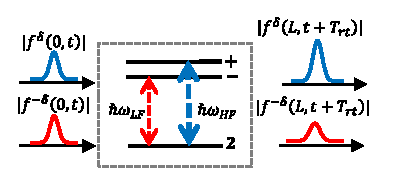
\includegraphics[scale=1.1]{IMGS/THB_pulse_interaction.eps}
		\caption{ Insert Caption HERE} \label{fig:img03}
	\end{center}	
\end{figure}
Upon propagation through the active region, if they are broad enough, both pulses "see" the same gain shape, i.e. they see both spectral lobes of the gain with it's spectral hole due to anticrossing. However, they do not interact with the medium equally, but rather with strength proportional to the dipole matrix elements $d_{\pm c} = \bra{\pm}\h{z}\ket{c}$, which, as has been shown before [cite our paper] \cite{dupont2010simplified}, depends upon the bias around injector $\leftrightarrow$ upper laser level resonance. If we consider a situation where the high frequency lobe has higher gain, then upon a single propagation through a cavity of length $L$, the positive frequency envelope $f^{\delta}$ will be amplified stronger than $f^{-\delta}$, as schematically illustrated in Fig. \ref{fig:img03}. This conclusion can be in fact confirmed by performing a computational version of THz time domain spectroscopy [CITE PAPERS],  where the input and output signals at $x=0$ and $x=L$ are recorded and the acquired phase shift and amplification ratios readily computed by manipulating their Fourier transforms [cite our paper]. In fact, we find this as quite a convenient method for gain and dispersion characterization of arbitrarily complex systems, modelled via the density matrix formalism, as it gives us access to the linear and nonlinear properties of the material, without having to resort to tedious analytical calculations or adhere to any steady state assumptions. 

Results from one such numerical "experiment" for a high and low frequency pulse, propagating through a cavity with length $L = 2.5$ mm of a gain medium modelled after the device in Ref \cite{burghoff2014terahertz}, are depicted in Fig. \ref{fig:img04}. The operating bias throughout the simulation was set a little below $b\leftrightarrow c$ resonance, i.e. $\epsilon <0$, at 10.8 kV/cm. The rest of the model parameters, e.g. the scattering rates, eigenenergies, anticrossing strengths etc. could be found elsewhere [cite optics express paper].
\begin{figure}[h!]
	\begin{center}
		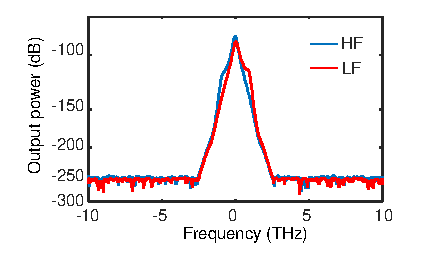
\includegraphics[scale=1.0]{IMGS/THzTDs.eps}
		\caption{ Insert Caption HERE} \label{fig:img04}
	\end{center}	
\end{figure}

Fig. \ref{fig:img04} depicts a log plot of the output amplitude spectrum of the high and low frequency lobes upon a single propagation through the cavity. We first notice that both curves are centred around zero, which is a consequence of our ansatz in Eq. (\ref{eq:field_ansatz}), which subtracts the leading positive and negative frequency components. Furthermore, since the simulation was performed a little below resonance, $f^{+\delta}$ experiences higher gain and is thus amplified more.  

What is important to note here is that both spectral components compete for the same gain. This is evident by the fact that the output power spectrum in Fig. \ref{fig:img04} has small "bumps" a
  
\appendix[The temporal hole burning equations]
\label{a:appendix01}

\begin{figure*}[!t]
	% ensure that we have normalsize text
	\normalsize
	% Store the current equation number.
	% Set the equation number to one less than the one
	% desired for the first equation here.
	% The value here will have to changed if equations
	% are added or removed prior to the place these
	% equations are referenced in the main text.
	%\setcounter{equation}{5}
	\begin{subequations}
		\label{eq:mainsystem}
	\begin{align}
	\label{eq:temporal-hole-11}
	\frac{d\rho_{cc}^{DC}}{dt} &= i\Omega_{cb}(\rho_{cb}^{DC}-(\rho_{cb}^{DC})^*) +  \Gamma_{bc}\rho_{bb}^{DC} + \Gamma_{ac}\rho_{aa}^{DC}  -\Gamma_{c}\rho_{cc}^{DC}, \\
	\frac{d\rho_{cc}^{+}}{dt} &= 2i\delta\omega\rho_{cc}^{+} + i\Omega_{cb}(\rho_{cb}^{+}-(\rho_{cb}^{-})^*) +  \Gamma_{bc}\rho_{bb}^{+} + \Gamma_{ac}\rho_{aa}^{+}  -\Gamma_{c}\rho_{cc}^{+}, \\
	\label{eq:temporal-hole-bb}
	\frac{d\rho_{bb}^{DC}}{dt} &= -i\Omega_{cb}(\rho_{cb}^{DC}-(\rho_{cb}^{DC})) + i\frac{q_0d_{ba}}{2\hbar} \left [ ( f^{(\delta)})^*\eta_{ba}^{(\delta)} +(f^{(-\delta)})^*\eta_{ba}^{(-\delta)} -c.c.\right]
	+\Gamma_{cb}\rho_{cc}^{DC} + \Gamma_{ab}\rho_{aa}^{DC} - \Gamma_b \rho_{bb}^{DC}, \\
	\frac{d\rho_{bb}^{+}}{dt} &= 2i\delta\omega\rho_{bb}^{+} - i\Omega_{cb}(\rho_{cb}^{+}-(\rho_{cb}^{-})^*) + i\frac{q_0d_{ba}}{2\hbar} \left [ (f^{(-\delta)})^*\eta_{ba}^{(\delta)} -f^{(\delta)}(\eta_{ba}^{(-\delta)})^*\right]
	+\Gamma_{cb}\rho_{cc}^{+} + \Gamma_{ab}\rho_{aa}^{+} - \Gamma_b \rho_{bb}^{+}, \\
	\frac{d\rho_{aa}^{DC}}{dt} &= -i\frac{q_0d_{ba}}{2\hbar} \left [ ( f^{(\delta)})^*\eta_{ba}^{(\delta)} +(f^{(-\delta)})^*\eta_{ba}^{(-\delta)} -c.c.\right]
	+\Gamma_{ca}\rho_{cc}^{DC} + \Gamma_{ba}\rho_{bb}^{DC} - \Gamma_a \rho_{aa}^{DC}, \\
	\frac{d\rho_{aa}^{+}}{dt} &= 2i\delta\omega\rho_{aa}^{+} - i\frac{q_0d_{ba}}{2\hbar} \left [ (f^{(-\delta)})^*\eta_{ba}^{(\delta)} -f^{(\delta)}(\eta_{ba}^{(-\delta)})^*\right]
	+\Gamma_{ca}\rho_{cc}^{+} + \Gamma_{ba}\rho_{bb}^{+} - \Gamma_a \rho_{aa}^{+}, \\
	\frac{d \rho_{cb}^{DC}}{d t}  &= -i\epsilon\rho_{cb}^{DC} +i \Omega_{cb}(\rho_{cc}^{DC} - \rho_{bb}^{DC}) +i\frac{q_0d_{ba}}{2 \hbar}((f^{(\delta)})^*\eta_{ca}^{(\delta)} +(f^{(-\delta)})^*\eta_{ca}^{(-\delta)})
	-\Gamma_{\parallel cb} \rho_{cb}^{DC},  \\
	\frac{d \rho_{cb}^{\pm}}{d t}  &= -i(\epsilon \mp 2\delta\omega)\rho_{cb}^{+} +i \Omega_{cb}(\rho_{cc}^{\pm} - \rho_{bb}^{\pm}) +i\frac{q_0d_{ba}}{2 \hbar}( (f^{(\mp\delta)})^*\eta_{ca}^{(\pm\delta)} )- \Gamma_{\parallel cb} \rho_{cb}^{\pm},\\
	\frac{d \eta_{ba}^{(\pm\delta)}}{d t} &= -i(\Delta \mp \delta\omega)\eta_{ba}^{(\pm\delta)}
	+i\frac{q_0d_{ba}}{2\hbar} \left[ f^{(\pm\delta)}(\rho_{bb}-\rho_{aa})^{DC} + f^{(\mp \delta)} (\rho_{bb}^{\pm}-\rho_{aa}^{\pm})\right]-i\Omega_{cb}\eta_{ca}^{(\pm\delta)}- \Gamma_{\parallel ba}\eta_{ba}^{(\pm\delta)}, \label{eq:eta_cb-temphole} \\
	\frac{d \eta_{ca}^{(\pm\delta)}}{d t} &= -i(\Delta+\epsilon \mp \delta\omega)\eta_{ca}^{(\pm\delta)}+i\frac{q_0d_{ba}}{2\hbar} ( f^{(\pm\delta)}\rho_{cb}^{DC} + f^{(\mp \delta)} \rho_{cb}^{\pm})-i\Omega_{cb}\eta_{ba}^{(\pm\delta)}-
	\Gamma_{\parallel ca}\eta_{ca}^{(\pm\delta)}, \label{eq:eta_ca-temphole}
	\end{align} 
	\end{subequations}
	% Restore the current equation number.
	% IEEE uses as a separator
	\hrulefill
	% The spacer can be tweaked to stop underfull vboxes.
	\vspace*{4pt}
\end{figure*}

The coefficients $\Gamma_{ij} $ are the scattering rates from state $\ket{i}$ to state $\ket{j}$, $\Gamma_k = \sum_{j}\Gamma_{kj}$ is the total out-scattering rate from level $\ket{k}$ and $\Gamma_{\parallel ij} = \frac{1}{2}(\Gamma_{i} + \Gamma_j) + \Gamma_{i,j}^*$ with $\Gamma_{i,j}^*$ the pure dephasing rate for the transition $i\rightarrow j$ and we have include a linear power loss term $l_0$ in the envelope propagation equations. 
Finally, we expand the wave propagation equations Eq. (\ref{eq:rtwave}) and see that the high and low frequency lobes' envelopes satisfy
\begin{align}
\frac{n}{c}\partial_t f^{(\pm \delta)} + \partial_{x}f^{(\pm \delta)}&= -i\frac{N \Gamma q_0d_{ba} k_c}{\epsilon_0 n^2} \eta_{ba}^{(\pm \delta)}  \nonumber \\ 
&-\left[\frac{l_0}{2}  \mp i (\frac{n\delta\omega}{c}-\delta k)\right] f^{(\pm \delta)}\label{eq:rtwave-temphole}.
\end{align}


% References <- adhere to respective journal style 
\bibliographystyle{IEEEtran}
\bibliography{D:/docs/Paper/literature/bib_resources}


\end{document} 
